\documentclass[class=article,crop=false]{standalone} \usepackage[margin=1in,headheight=57pt,headsep=0.1in]{geometry}
\usepackage[subpreambles=true]{standalone}
\usepackage{float}
\usepackage[framemethod=TikZ]{mdframed}
\usepackage{fancyhdr}
\usepackage[utf8]{inputenc} % Required for inputting international characters
\usepackage[T1]{fontenc} % Output font encoding for international characters
\usepackage{stix} % Use the STIX fonts
\usepackage{hyperref}
\hbadness=99999

\begin{document}
\subsection{The Main Menu Form}
\begin{figure}[H]
	\centering
	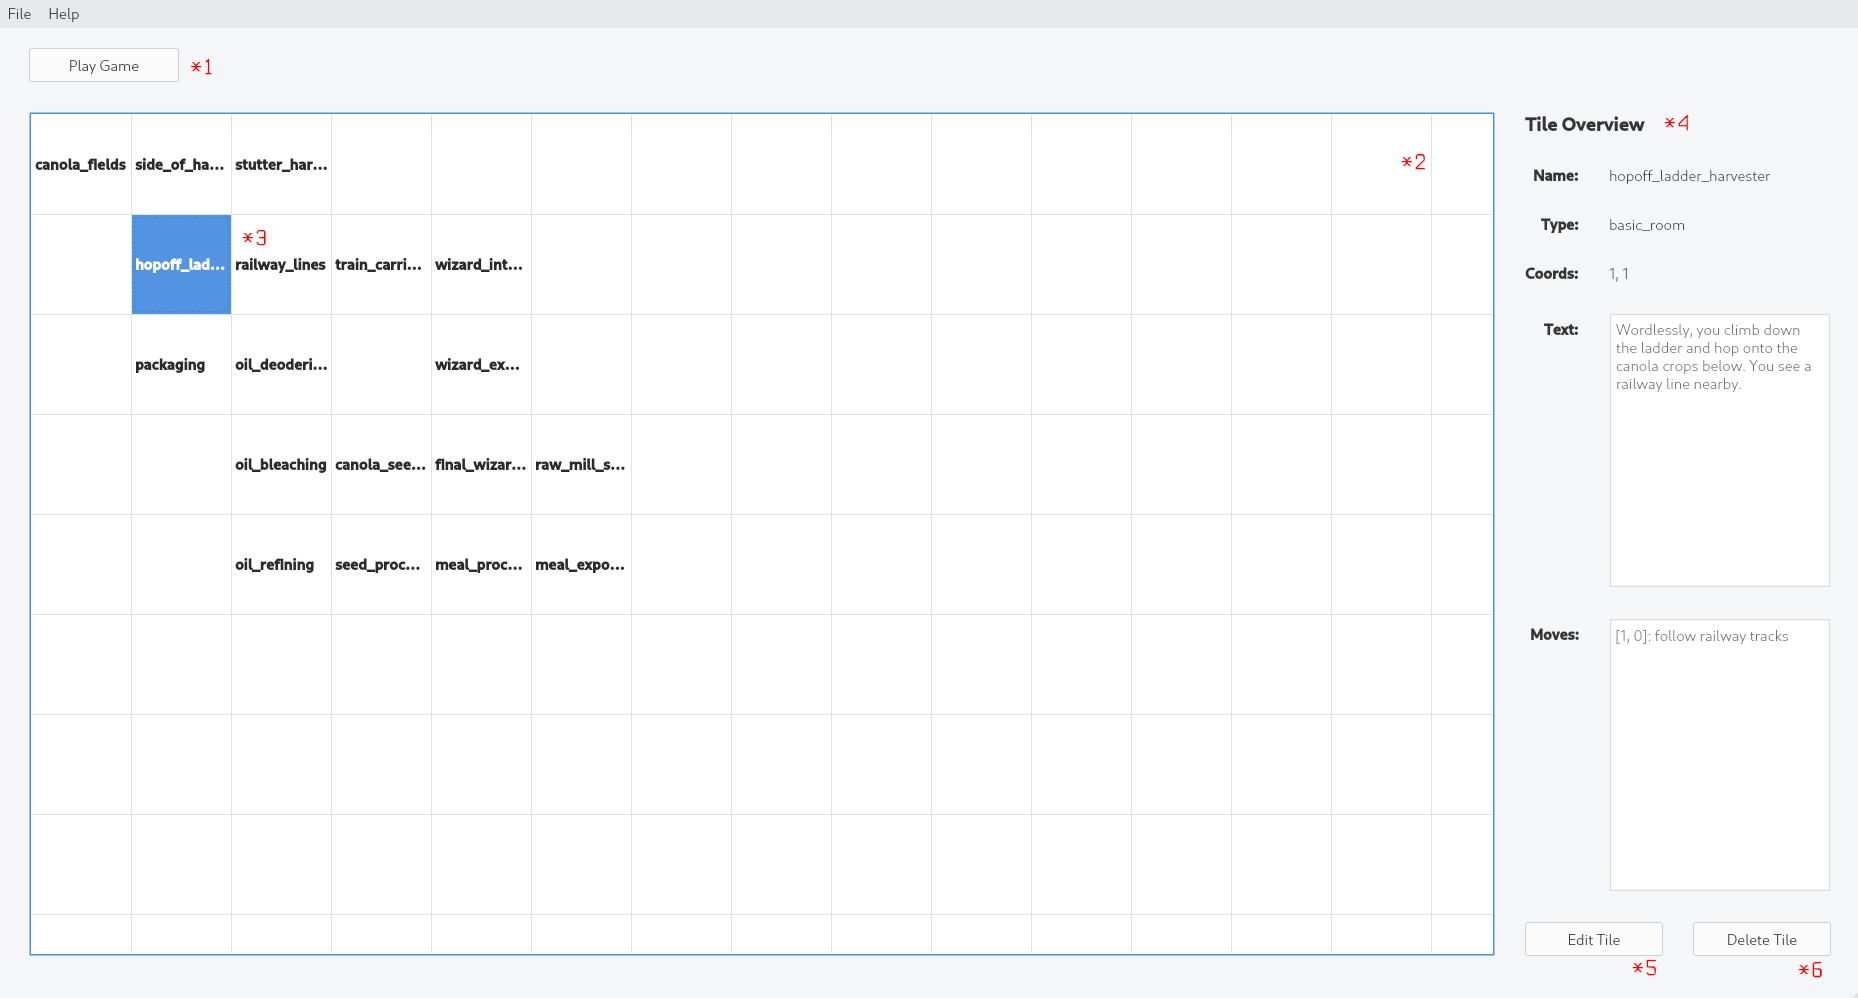
\includegraphics[width=1.0\textwidth]{./mainMenuForm.png}
\end{figure}
This is the main form of \texttt{tbrpggepp}. The elements in this screenshot are labelled as follows:
\begin{enumerate}
	\item "Play Game" button. This opens a terminal in a new window running the text-based game, allowing you to play out your narrative.
	\item The game-world grid. This grid essentially provides a top-down view of the "world" for your text-based game, consisting of hundreds of invisible, empty "tiles" which you may edit and populate with data for the player to interact with. Within this screenshot we see many tiles have already been created and populated with data, thus creating a short text-based adventure. \textbf{Note that at the beginning of every game the player always starts at the topmost leftmost tile, which has coordinates of 0,0.}
	\item You may click on a populated or empty tile to interact with it or view its contents. In this screenshot we see a populated tile has been selected, displaying its contents in the sidebar and allowing the user to either edit it or delelete it by clicking the appropriate buttons.
	\item The sidebar ie. Tile Overview. This presents a read-only view of the contents of the selected tile, including the following elements:
		\begin{itemize}
			\item Name: the unique identifier for a tile, unseen by the player but cannot be reused.
			\item Type: the category of tile, which defines how the user interacts with it. Categories include \texttt{basic\_room} (simply displays text), \texttt{enemy\_room} (contains an enemy for the player to fight), \texttt{item\_room} (contains an item that the player picks up), and \texttt{victory\_room} (identical to a basic tile, except the game ends after the player enters it).
			\item Coords: the X and Y coordinate values of the tile (in that order), representing the tile's location within the game-world.
			\item Text: the words that the player sees upon entering a tile of any type for the first time.
			\item Moves: an overview of the methods in which the player can navigate out of the selected tile. Displays a "coordinate delta" and "label" for each move. The label is simply what the player enters to conduct the move. The "coordinate delta" mathematically represents the change in coordinates applied to the player after conducting the move. For example, a player residing in coordinates 1,1 with a move of [1,0] applied to them would end up in 2,1; which is one unit to the right on the game-world grid. For another example, applying the move [0,-1] on a player residing in 2,6 would move them to 2,5; which is one unit upwards on the game-world grid.
		\end{itemize}
	\item "Edit Tile" button. Clicking this opens the Edit Tile form, allowing you to edit the contents of the currently selected tile. If an empty tile was initially selected then a new tile will be created at its coordinates.
	\item "Delete Tile" button. Clicking this will turn the currently selected tile into an empty tile, handle with care!
	\item An additional element is the "file" menu option in the upper left: this allows you to re-open the Introduction form and open/create a different world file. The "help" option simply links to relevant pages of this document.
\end{enumerate}
\subsubsection{Playing the Game}
As stated above, clicking the "Play Game" button in the Main Menu form will open a terminal in a new window that is running the text-based game. A screenshot of one such terminal is provided below:
\begin{figure}[H]
	\centering
	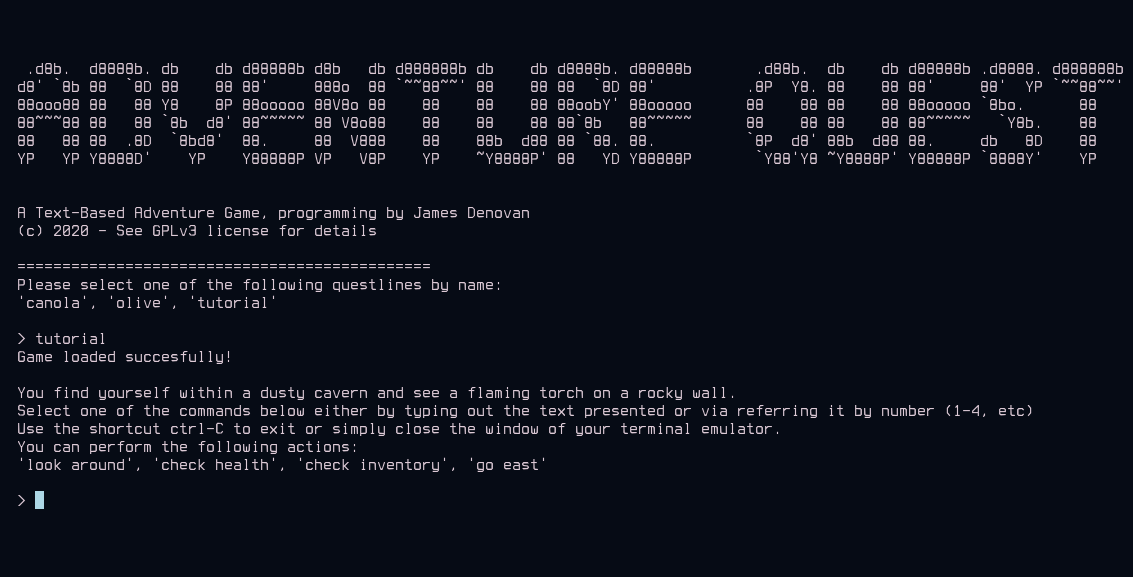
\includegraphics[width=1.0\textwidth]{./gameplay.png}
\end{figure}
When the game program begins, it gives you the decision to choose any of the other game-world files within the directory of your \texttt{tbrpggepp} world file. After loading the desired game-world file, we see the player met with the introductory text of the tile at coordinates 0,0; followed by a prompt where the player may either:
\begin{itemize}
	\item "\texttt{look around}": displays the text in the "Description" field shown in the Edit Tile Form section.
	\item "\texttt{check health}": displays the current HP (Health Points) value of the player
	\item "\texttt{check inventory}": displays the current inventory of the player
	\item "\texttt{go east}": evidently one of the moves created for the tile at coordinates 0,0.
\end{itemize}
Other scenarios display different prompts, such as when one has consumable health items in their inventory or are engaged in a battle with an enemy. This "tutorial" questline is provided alongside \texttt{tbrpggepp}, which you may want to attempt in order to gain familiarity with \texttt{Adventure Quest}'s style of gameplay.
\end{document}
